\documentclass{article}
\usepackage{natbib}

% if you need to pass options to natbib, use, e.g.:
%     \PassOptionsToPackage{numbers, compress}{natbib}
% before loading neurips_2022


% ready for submission
\usepackage{neurips_2022}

% to compile a preprint version, e.g., for submission to arXiv, add add the
% [preprint] option:
%     \usepackage[preprint]{neurips_2022}


% to compile a camera-ready version, add the [final] option, e.g.:
%     \usepackage[final]{neurips_2022}


% to avoid loading the natbib package, add option nonatbib:
%    \usepackage[nonatbib]{neurips_2022}


\usepackage[utf8]{inputenc} % allow utf-8 input
\usepackage[T1]{fontenc}    % use 8-bit T1 fonts
\usepackage{hyperref}       % hyperlinks
\usepackage{url}            % simple URL typesetting
\usepackage{booktabs}       % professional-quality tables
\usepackage{amsfonts}       % blackboard math symbols
\usepackage{nicefrac}       % compact symbols for 1/2, etc.
\usepackage{microtype}      % microtypography
\usepackage{xcolor}         % colors
\usepackage{graphicx}       % 图片支持
\usepackage{ctex}           % 中文支持
\usepackage{amsmath}        % 公式支持
\usepackage{multirow}       % 多行合并
\usepackage{makecell}       % 单元格内换行
\usepackage{float}          % 图表位置固定
\usepackage{subfigure}      % 子图支持
\usepackage{caption}        % 图表标题
\usepackage{listings}       % 代码支持
\usepackage{algorithm}      % 算法框架
\usepackage{algpseudocode}  % 伪代码
\usepackage{amssymb}        % 数学符号
\usepackage{bm}             % 数学符号加粗
\usepackage{amsthm}         % 定理环境
\usepackage{enumitem}       % 列表定制
\usepackage{diagbox}        % 表头斜线
\usepackage{array}          % 表格固定宽度
\usepackage{longtable}      % 长表格


\title{数值代数大作业}
\bibliographystyle{plainnat} % 选择引用样式,可以是 plain、abbrv、unsrt 等

% The \author macro works with any number of authors. There are two commands
% used to separate the names and addresses of multiple authors: \And and \AND.
%
% Using \And between authors leaves it to LaTeX to determine where to break the
% lines. Using \AND forces a line break at that point. So, if LaTeX puts 3 of 4
% authors names on the first line, and the last on the second line, try using
% \AND instead of \And before the third author name.


\author{%
  高以恒 \\
  \texttt{2200010851@stu.pku.edu.cn} \\
  \texttt{cpu: M1 Pro} \\
  % examples of more authors
  % \And
  % Coauthor \\
  % Affiliation \\
  % Address \\
  % \texttt{email} \\
  % \AND
  % Coauthor \\
  % Affiliation \\
  % Address \\
  % \texttt{email} \\
  % \And
  % Coauthor \\
  % Affiliation \\
  % Address \\
  % \texttt{email} \\
  % \And
  % Coauthor \\
  % Affiliation \\
  % Address \\
  % \texttt{email} \\
}

\newcommand{\figref}[1]{图\ref{#1}}
\newcommand{\tabref}[1]{表\ref{#1}}
\newcommand{\equref}[1]{式\ref{#1}}
\newcommand{\secref}[1]{第\ref{#1}节}


\begin{document}


\maketitle

\section{问题描述}
考虑Stokes方程
\begin{equation}
  \left\{\begin{aligned}
  -\Delta \vec{u}+\nabla p & =\vec{F}, & (x, y) & \in(0,1) \times(0,1) \\
  \operatorname{div} \vec{u} & =0, & (x, y) & \in(0,1) \times(0,1)
  \end{aligned}\right. \\
\end{equation}
边界条件为
\begin{equation*}
  \begin{aligned}
    \frac{\partial u}{\partial \vec{n}}&=b, & y & =0, & \frac{\partial u}{\partial \vec{n}}&=t, & y & =1, \\
    \frac{\partial v}{\partial \vec{n}}&=l, & x & =0, & \frac{\partial v}{\partial \vec{n}}&=r, & x & =1, \\
    u & =0, & x & =0,1, &
    v & =0, & y & =0,1
    \end{aligned}
\end{equation*}
其中$\vec{u}=(u, v)$是速度场,$p$是压力场,$\vec{F}=(f, g)$是外力场,$\vec{n}$是单位外法向量。
利用交错网格上的MAC格式离散方程(1),可得如下线性方程组
\begin{equation}
  \begin{pmatrix}
    A & B \\
    B^{T} & 0
  \end{pmatrix}
  \begin{pmatrix}
    U \\
    P
  \end{pmatrix}
  =
  \begin{pmatrix}
    \vec{F} \\
    0
  \end{pmatrix}
\end{equation}
具体形式见附录。

在该例中,外力为
\begin{equation*}
  \begin{aligned}
    f(x, y)&=-4\pi^{2}(2\cos(2\pi x)-1)\sin(2\pi y)+x^2, \\
    g(x, y)&=4\pi^{2}(2\cos(2\pi y)-1)\sin(2\pi x).
  \end{aligned}
\end{equation*}
Stokes方程(1)的解析解为
\begin{equation*}
  \begin{aligned}
    u(x, y)&=(1-cos(2\pi x))\sin(2\pi y), \\
    v(x, y)&=-(1-cos(2\pi y))\sin(2\pi x), \\
    p(x, y)&=\frac{x^3}{3}-\frac{1}{12}.
  \end{aligned}
\end{equation*}
其中压力$p$的取值可能有任意常数的平移。

\section{Task1}

分别取 N = 64, 128, 256, 512, 1024, 2048, 以 DGS 为磨光子, 用基于 V-cycle 的多重网格
方法求解离散问题 (2), 停机标准为 $\|r_h\|_{2} / \|r_{0}\|_{2} \leq 10^{-8}$。
对不同的 $v1,v2,L$, 比较 V-cycle 的次数和 CPU 时间, 并计算误差
$$
e_{N} = h \left( \sum_{j=1}^{N} \sum_{i=1}^{N} \left( u_{i,j-\frac{1}{2}} - u(x_i,y_{j-\frac{1}{2}}) \right)^{2} + \sum_{j=1}^{N-1} \sum_{i=1}^{N-1} \left( v_{i-\frac{1}{2},j} - v(x_{i-\frac{1}{2}},y_j) \right)^{2} \right)^{\frac{1}{2}}
$$

\subsection{DGS迭代法和V-cycle多重网格方法}
给定初始值$U_0,P_0 = p_0,f,g$,迭代格式如下:
1. 用Gauss-Seidel迭代法求解$AU^{(k+1)} = F - B^{T}P^{(k)}$,得到$U^{(k+1/2)}$;
2. 更新内部速度和压力:
\begin{equation}
  \begin{aligned}
    U^{(k+1)} &= U^{(k+1/2)} + B (B^T B)^{-1} (g - B U^{(k+1/2)}), \\
    P^{(k+1)} &= P^{(k)} - (g - B U^{(k+1/2)}).
  \end{aligned}
\end{equation}

\begin{algorithm}
  \caption{V-cycle多重网格方法}
  \begin{algorithmic}[1]
    \Require $U_0, P_0, f, g, v1, v2, N, L$
    \Ensure 解 $U_h$ 和 $P_h$
    \State 初始化残差 $r_h = f - A_h U_h$
    \While{$\|r_h\|_{2} / \|r_{0}\|_{2} > 10^{-8}$}
      \State 对 $U_h$ 和 $P_h$ 进行 $v1$ 次 DGS 更新
      \If{$L == N$}
        \State \Return $U_h, P_h$
      \Else
        \State 将残差 $r_h$ 限制到粗网格:$r_{2h} = R(r_h)$
        \State 初始化粗网格解:$U_{2h} = 0$, $P_{2h} = 0$
        \State 递归调用 V-cycle($U_{2h}, P_{2h}, r_{2h}, f_{2h}, g_{2h}, v1, v2, 2h, L+1$)
        \State 将粗网格解插值回细网格:$U_h = U_h + I(U_{2h})$, $P_h = P_h + I(P_{2h})$
      \EndIf
      \State 对 $U_h$ 和 $P_h$ 进行 $v2$ 次 DGS 更新
      \State 更新残差:$r_h = f - A_h U_h$
    \EndWhile
  \end{algorithmic}
\end{algorithm}

注:在计算粗网格上的$A_{2h},B_{2h}$时,按照课件上的方法,$A_{2h},B_{2h}$的形式如下:
\begin{equation*}
  \begin{pmatrix}
    A_{2h} & B_{2h} \\
    B_{2h}^{T} & 0
  \end{pmatrix}
  =
  I_{h}^{2h}
  \begin{pmatrix}
    A_h & B_h \\
    B_h^{T} & 0
  \end{pmatrix}
  I_{2h}^{h}
\end{equation*}
其中$I_{h}^{2h}$是限制算子,$I_{2h}^{h}$是插值算子。
但是这样做的计算代价比较大:一方面要进行矩阵乘法,另一方面得到的$A_{2h},B_{2h}$的稀疏性比较差。
因此,在具体实现中我们直接用粗网格上的MAC格式离散得到的稀疏矩阵去近似,实际效果也是比较好的。
如果想使用前一种方法,我也提供了选项,具体参见代码。

考虑到在粗网格上进行迭代的时间复杂度较低,在实际实现中我让$v2 = v_{20} + log_2(N_0/N)$,其中$v_{20}$是在初始网格上进行迭代的次数,$N_0$是初始网格的大小。

\subsection{并行加速}

对DGS,两部分更新都可以并行化,这里使用OpenMP对细网格$(N>8)$进行并行加速。
对Gaussian-Seidel迭代法,使用红黑着色法,将网格分为红色和黑色两部分,分别更新。
对压力和速度的更新,可以简单的分成8个部分,分别更新。

\subsection{数值结果}
对不同的迭代次数$v1,v2$和底层网格大小$N$,得到的误差误差很小,因此只给出$v1 = 3, v2 = 1, N/L = 2$时的结果。

\begin{table}[!h]
  \centering
  \begin{tabular}{cccccccc}
    \toprule
    $N$ & 64 & 128 & 256 & 512 & 1024 & 2048 & 4096 \\
    \midrule
    误差 & 1.4951e-3 & 3.7363e-4 & 9.3399e-5 & 2.3349e-5 & 5.8372e-6 & 1.4593e-6 & 3.6480e-7 \\
    \bottomrule
  \end{tabular}
\end{table}


对不同迭代次数和底层网格大小的运行时间和V-cycle迭代次数比较:

\begin{table}[!h]
  \centering
  \caption{$v1 = 1, v2 = 3, N/L = 2$}
  \setlength{\belowcaptionskip}{-5pt} 
  \begin{tabular}{cccccccc}
    \toprule
    $N$ & 64 & 128 & 256 & 512 & 1024 & 2048 \\
    \midrule
    迭代次数 & 6 & 6 & 6 & 6 & 6 & 6 \\
    CPU时间 & 0.0378 & 0.0396 & 0.0845 & 0.2574 & 0.8284 & 3.4668 \\
    \bottomrule
  \end{tabular}
\end{table}
注:时间复杂度是$O(N^2)$的,对于4096的网格,由于16g内存限制,部分数据需要存储在硬盘上,因此时间较长(30s)。实测在64g内存的机器上,8192的网格也可以在80s左右完成。

\begin{table}[!h]
  \centering
  \caption{$v1 = 1, v2 = 3, N/L = 4$}
  \begin{tabular}{cccccccc}
    \toprule
    $N$ & 64 & 128 & 256 & 512 & 1024 & 2048 \\
    \midrule
    迭代次数 & 6 & 6 & 6 & 6 & 6 & 6 \\
    CPU时间 & 0.0345 & 0.0581 & 0.1125 & 0.3260 & 0.9912 & 3.6560 \\
    \bottomrule
  \end{tabular}
\end{table}
\vspace{-10pt}
\begin{table}[!h]
  \centering
  \caption{$v1 = 1, v2 = 1, N/L = 2$}
  \begin{tabular}{cccccccc}
    \toprule
    $N$ & 64 & 128 & 256 & 512 & 1024 & 2048 \\
    \midrule
    迭代次数 & 9 & 9 & 9 & 9 & 9 & 9 \\
    CPU时间 & 0.0399 & 0.0407 & 0.0945 & 0.3062 & 0.9557 & 4.1706  \\
    \bottomrule
  \end{tabular}
\end{table}

\begin{table}[!h]
  \centering
  \caption{$v1 = 1, v2 = 1, N/L = 4$}
  \begin{tabular}{cccccccc}
    \toprule
    $N$ & 64 & 128 & 256 & 512 & 1024 & 2048 \\
    \midrule
    迭代次数 & 9 & 9 & 9 & 9 & 9 & 9 \\
    CPU时间 & 0.0246 & 0.0429 & 0.0975 & 0.2850 & 1.0103 & 4.2779  \\
    \bottomrule
  \end{tabular}
\end{table}

\begin{table}[!h]
  \centering
  \caption{$v1 = 2, v2 = 2, N/L = 2$}
  \begin{tabular}{cccccccc}
    \toprule
    $N$ & 64 & 128 & 256 & 512 & 1024 & 2048  \\
    \midrule
    迭代次数 & 6 & 6 & 6 & 6 & 6 & 6  \\
    CPU时间 & 0.0276 & 0.0375 & 0.0872 & 0.2694 & 0.8494 & 3.5884 \\
    \bottomrule
  \end{tabular}
\end{table}

\begin{table}[!h]
  \centering
  \caption{$v1 = 2, v2 = 2, N/L = 4$}
  \begin{tabular}{cccccccc}
    \toprule
    $N$ & 64 & 128 & 256 & 512 & 1024 & 2048  \\
    \midrule
    迭代次数 & 6 & 6 & 6 & 6 & 6 & 6  \\
    CPU时间 & 0.0345 & 0.0581 & 0.1125 & 0.3260 & 0.9912 & 3.6560  \\
    \bottomrule
  \end{tabular}
\end{table}

\begin{table}[!h]
  \centering
  \caption{$v1 = 3, v2 = 3, N/L = 2$}
  \begin{tabular}{cccccccc}
    \toprule
    $N$ & 64 & 128 & 256 & 512 & 1024 & 2048 \\
    \midrule
    迭代次数 & 6 & 6 & 6 & 6 & 6 & 6  \\
    CPU时间 & 0.0374 & 0.0490 & 0.1167 & 0.3090 & 0.9741 & 4.0411  \\
    \bottomrule
  \end{tabular}
\end{table}

\begin{table}[!h]
  \centering
  \caption{$v1 = 3, v2 = 3, N/L = 4$}
  \begin{tabular}{cccccccc}
    \toprule
    $N$ & 64 & 128 & 256 & 512 & 1024 & 2048 \\
    \midrule
    迭代次数 & 6 & 6 & 6 & 6 & 6 & 6  \\
    CPU时间 & 0.0465 & 0.0473 & 0.1063 & 0.3131 & 1.0737 & 4.3676  \\
    \bottomrule
  \end{tabular}
\end{table}
\newpage
更多结果见附录5.3. 可以看到,$v1, v2$的取值不需要太大,$N/L$的取值则为2时效果最好,这也符合V-cycle多重网格方法的特点。
理论上,算法的时间复杂度为$O(N^2)$,误差阶为$O(h^2)$,数值结果也符合这一点。

\section{Task2}

分别取 N = 64, 128, 256, 512, 以 Uzawa Iteration Method 求解离散问题(2), 停机标准为 $\|r_h\|_{2} / \|r_{0}\|_{2} \leq 10^{-8}$。
计算误差 $e_{N}$。

\subsection{Uzawa迭代法}
\begin{algorithm}
  \caption{Uzawa迭代法}
  \begin{algorithmic}[1]
    \Require $U_0, P_0, f, N, \alpha$
    \Ensure 解 $U_h$ 和 $P_h$
    \State 初始化残差 $r_h = f - A_h U_h$
    \While{$\|r_h\|_{2} / \|r_{0}\|_{2} > 10^{-8}$}
      \State 利用CG方法求解$A U_{k+1} = f - B^T P_k$
      \State 更新压力:$P_{k+1} = P_k + \alpha B U_{k+1}$
      \State 更新残差:$r_h = f - A_h U_h$
    \EndWhile
  \end{algorithmic}
\end{algorithm}

关于$\alpha$的选取,分析知$ B^T A^{-1} B$的特征值为0和1,因此$\alpha$的最佳取值为1.(见附录5.2)

\subsection{数值结果}
对CG算法的精确度要求为$10^{-9}$,对Uzawa迭代法的精确度要求为$10^{-8}$。
\begin{table}[!h]
  \centering
  \begin{tabular}{ccccc}
    \toprule
    $N$ & 64 & 128 & 256 & 512 \\
    \midrule
    迭代次数 & 2 & 2 & 2 & 2 \\
    CPU时间 & 0.0401 & 0.0958 & 0.8966 & 5.9550 \\
    误差 & 1.4951e-3 & 3.7363e-4 & 9.3399e-5 & 2.3349e-5 \\
    \bottomrule
  \end{tabular}
\end{table}

\section{Task3}

分别取 N = 64, 128, 256, 512, 1024, 2048, 以 Inexact Uzawa Iteration Method 为迭代法求
解离散问题 (2), 停机标准为 $\|r_h\|_{2} / \|r_{0}\|_{2} \leq 10^{-8}$。
其中以 V-cycle 多重网格方法为预条件子,
利用共轭梯度法求解每一步的子问题 $AU_{k+1} = F - B^{T}P_{k}$, 对不同的 $\alpha, \tau, \nu_1, \nu_2, L$, 比较外循环
的迭代次数和 CPU 时间, 并计算误差。

\subsection{Inexact Uzawa迭代法和V-cycle-PCG算法}

\begin{algorithm}[!h]
  \caption{Inexact Uzawa迭代法}
  \begin{algorithmic}[1]
    \Require $U_0, P_0, f, g, N, \alpha, \tau, \nu_1, \nu_2, L$
    \Ensure 解 $U_h$ 和 $P_h$
    \State 初始化残差 $r_h = f - A_h U_h$
    \While{$\|r_h\|_{2} / \|r_{0}\|_{2} > 10^{-8}$}
      \State 利用V-cycle-PCG方法求解$AU_{k+1} = f - B^T P_k$, 得到近似解$\hat{U}_{k+1}$,
      \State 更新压力:$P_{k+1} = P_k + \alpha B \hat{U}_{k+1}$
      \State 更新残差:$r_h = f - A \hat{U}_{k+1}$
    \EndWhile
  \end{algorithmic}
\end{algorithm}

定义$\delta_k = A \hat{U}_{k+1} - f + B^T P_k$, 若$\|\delta_k\|_2 \leq \tau \|B^T \hat{U}_{k+1}\|_2$,且$\tau$充分小,则上述方法收敛。

\begin{algorithm}[!h]
  \caption{V-cycle-PCG算法}
  \begin{algorithmic}[1]
    \Require: x
    \State $k=0, r = b - A x, \rho = r^T r$
    \While{$(\|r\|>max(\epsilon \|b\|,\tau\|B^T\hat{U}_k\| ) and k<K_max)$}
      \State $k = k + 1$
      \State 以GS迭代法为磨光子,利用V-cycle多重网格方法求解$Az = r$
      \If{$k=1$} 
        $p = z; \rho = z^T r$
      \Else
        $\rho_{old} = \rho; \rho = z^T r; \beta = \rho/\rho_{old}; p = z + \beta p$
      \EndIf
      \State $w = A p; \alpha = \rho/(p^T w); x = x + \alpha p; r = r - \alpha w$
    \EndWhile
  \end{algorithmic}
\end{algorithm}

该部分我尝试了对称GS迭代和红黑GS迭代,效果差不多,因此并行实现。
V-cycle多重网格算法停机标准为$\|r_h\|_{2} / \|r_{0}\|_{2} \leq 10^{-3} and k \leq 3$

\subsection{数值结果}
误差:

\begin{table}[!h]
  \centering
  \begin{tabular}{ccccccc}
    \toprule
    $N$ & 64 & 128 & 256 & 512 & 1024 & 2048 \\
    \midrule
    误差 & 1.4951e-3 & 3.7363e-4 & 9.3399e-5 & 2.3349e-5 & 5.8372e-6 & 1.4593e-6 \\
    \bottomrule
  \end{tabular}
\end{table}


\begin{figure}[!h]
  \centering
  \subfigure[$\alpha = 1, \tau = 10^{-3}$]{
    \begin{minipage}[t]{0.5\linewidth}
      \centering
      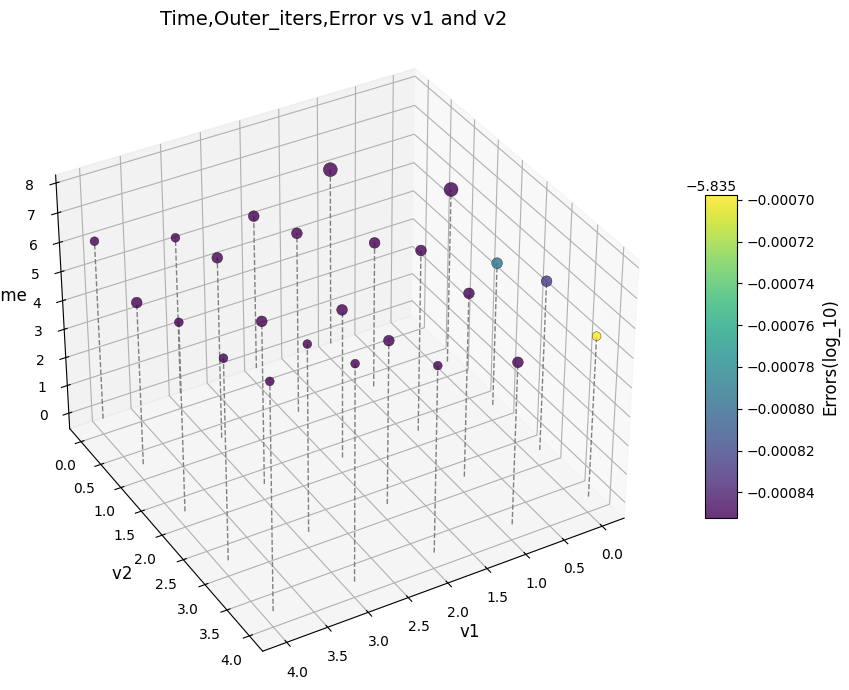
\includegraphics[width=2.7in]{v1v2.png}
    \end{minipage}%
  }%
  \subfigure[$\nu1 = 1, \nu2 = 1$]{
    \begin{minipage}[t]{0.5\linewidth}
      \centering
      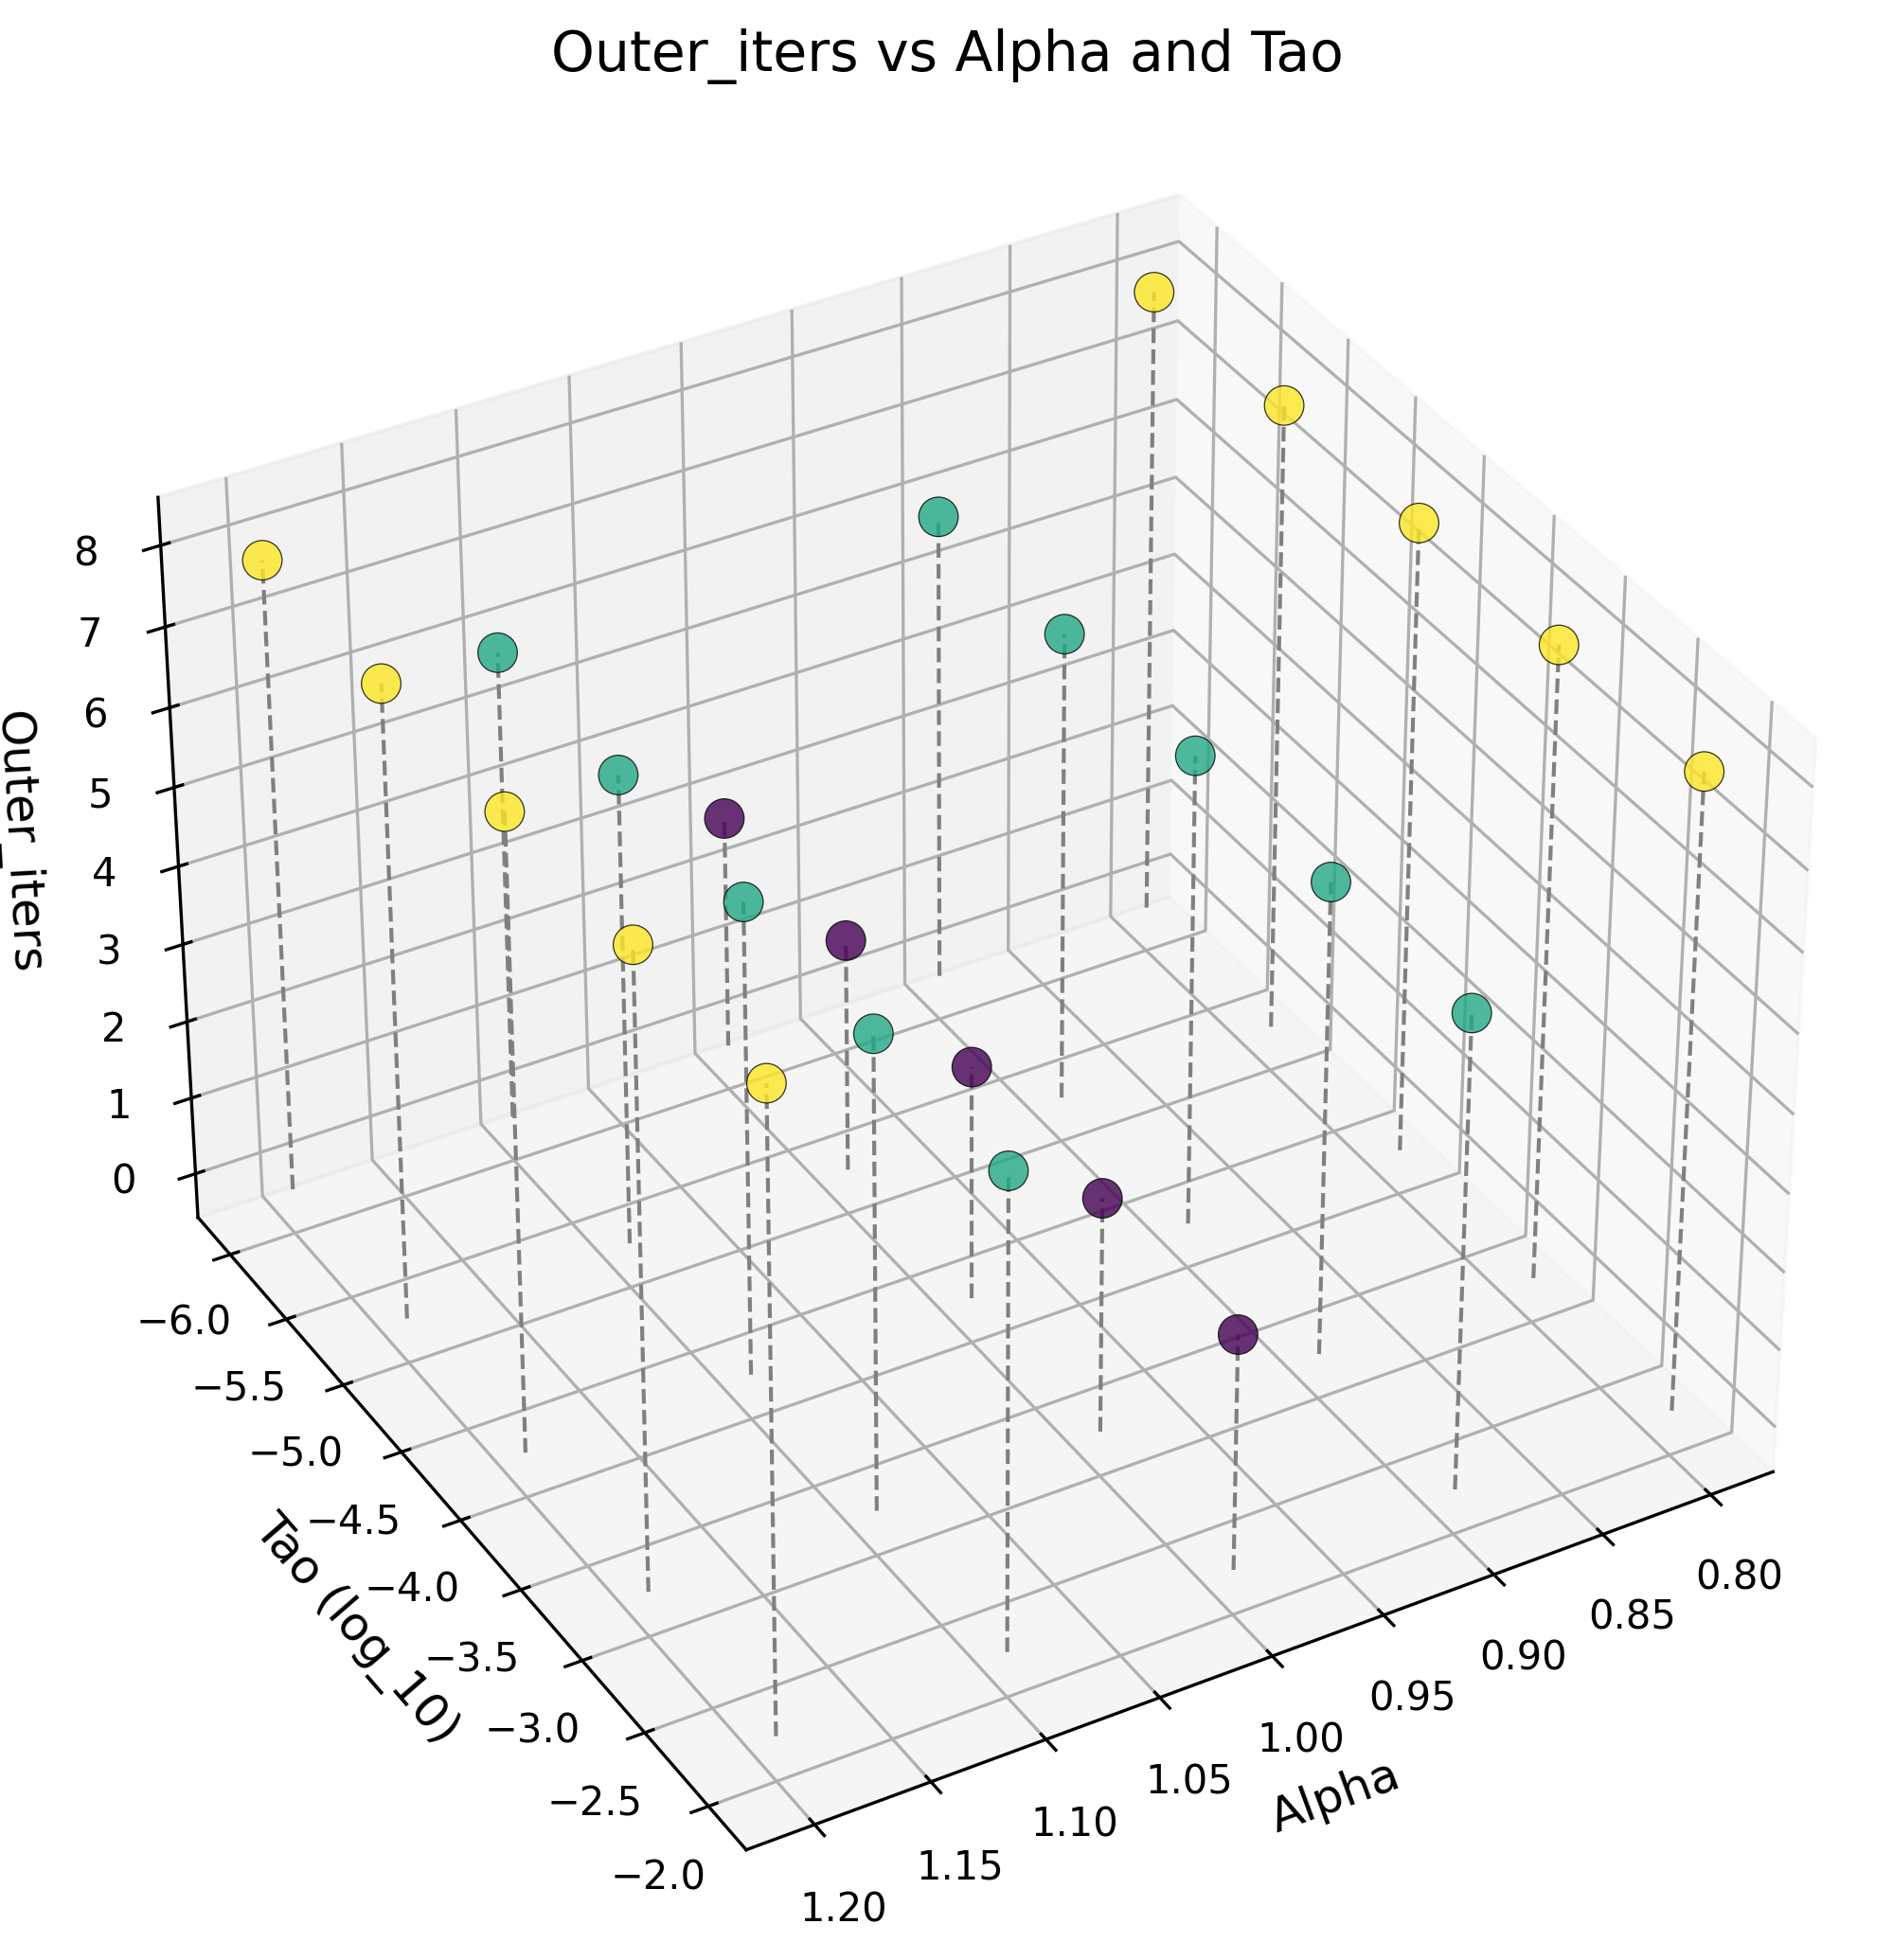
\includegraphics[width=2in]{alphatau.png}
    \end{minipage}%
  }%
  \caption{注:左图是cpu时间关于$v1,v2$的图,右图是外循环迭代次数关于$\alpha,\tau$的图。左图点的大小与迭代次数成正比,颜色表示误差大小。}
  \label{fig:1}
\end{figure}

不同参数对运行时间和V-cycle迭代次数的影响见\ref{fig:1}。这里分别固定$\alpha = 1, \tau = 10^{-3}$,$\nu1, \nu2$,改变另一组参数$(N/L=2,N=2048)$

可以看到,参数对改变对误差影响不大,但是对迭代次数和时间影响较大。
固定$\nu1,\nu2$,改变$\alpha,\tau$,可以看到$\alpha = 1$时效果最好,$\tau$取值对结果影响不大。

\newpage
最后以下给出几组组参数下的结果,该算法时间复杂度为$O(N^2)$,误差阶为$O(h^2)$,数值结果也符合这一点。
更多结果见附录。

$\alpha = 1, \tau = 10^{-3}, \nu1 = 1, \nu2 = 1, N/L = 2$:

\begin{table}[!h]
  \centering
  \begin{tabular}{ccccccc}
    \toprule
    $N$ & 64 & 128 & 256 & 512 & 1024 & 2048 \\
    \midrule
    CPU时间 & 0.0698 & 0.0579 & 0.1445 & 0.4214 & 1.2661 & 5.0848 \\
    Inexact Uzawa迭代次数 & 3 & 4 & 4 & 4 & 3 & 3 \\
    PCG迭代次数 & 3 3 2 & 3 2 1 1 & 3 2 1 1 & 3 2 1 1 & 3 2 1 & 2 3 1 \\
    \bottomrule
  \end{tabular}
\end{table}

$\alpha = 1, \tau = 10^{-3}, \nu1 = 1, \nu2 = 1, N/L = 4$:

\begin{table}[!h]
  \centering
  \begin{tabular}{ccccccc}
    \toprule
    $N$ & 64 & 128 & 256 & 512 & 1024 & 2048 \\
    \midrule
    CPU时间 & 0.1061 & 0.1597 & 0.3786 & 0.9168 & 2.7406 & 9.4641 \\
    Inexact Uzawa迭代次数 & 4 & 4 & 4 & 4 & 4 & 4 \\
    PCG迭代次数 & 5 15 2 1 & 4 14 2 1 & 4 12 2 1 & 3 11 2 1 & 3 9 2 1 & 3 8 2 1 \\
    \bottomrule
  \end{tabular}
\end{table}

$\alpha = 1, \tau = 10^{-3}, \nu1 = 2, \nu2 = 2, N/L = 2$:

\begin{table}[!h]
  \centering
  \begin{tabular}{ccccccc}
    \toprule
    $N$ & 64 & 128 & 256 & 512 & 1024 & 2048 \\
    \midrule
    CPU时间 & 0.0657 & 0.0730 & 0.1736 & 0.4687 & 1.5007 & 4.3087 \\
    Inexact Uzawa迭代次数 & 3 & 3 & 3 & 3 & 3 & 3 \\
    PCG迭代次数 & 3 3 1 & 3 3 1 & 3 3 1 & 3 3 1 & 3 3 1 & 2 2 1 \\
    \bottomrule
  \end{tabular}
\end{table}

$\alpha = 1, \tau = 10^{-3}, \nu1 = 2, \nu2 = 2, N/L = 4$:

\begin{table}[!h]
  \centering
  \begin{tabular}{ccccccc}
    \toprule
    $N$ & 64 & 128 & 256 & 512 & 1024 & 2048 \\
    \midrule
    CPU时间 & 0.1016 & 0.1409 & 0.2515 & 0.8003 & 1.9337 & 7.8004 \\
    Inexact Uzawa迭代次数 & 4 & 4 & 4 & 4 & 3 & 3 \\
    PCG迭代次数 & 3 8 2 1 & 3 6 2 1 & 3 5 1 1 & 3 3 2 1 & 3 4 1 & 3 3 1 \\
    \bottomrule
  \end{tabular}
\end{table}

\section{Appendix}

\subsection{交错网格上的MAC格式}
方程组(2)的系数矩阵$A,B$的具体形式如下:\\
$
  \begin{aligned}
    &\text{其中}A=
    \begin{pmatrix}
    A_{u} & \\
    & A_{v}
    \end{pmatrix},B=
    \begin{pmatrix}
    B_{u} \\
    B_{v}
    \end{pmatrix},A_{u},A_{v}\in\mathbb{R}^{N(N-1)\times N(N-1)}, \\
  \end{aligned}
$
\begin{equation*}
  \begin{aligned}
    & A_{u}=
    \begin{pmatrix}
    A_{1} & -\frac{1}{h^{2}}I \\
    -\frac{1}{h^{2}}I & A_{2} & -\frac{1}{h^{2}}I \\
    & -\frac{1}{h^{2}}I & A_{2} & -\frac{1}{h^{2}}I \\
    & & \ddots & \ddots & \ddots \\
    & & & -\frac{1}{h^{2}}I & A_{2} & -\frac{1}{h^{2}}I \\
    & & & & -\frac{1}{h^{2}}I & A_{1}
    \end{pmatrix},A_{v}=
    \begin{pmatrix}
    A_{3} & -\frac{1}{h^{2}}I \\
    -\frac{1}{h^{2}}I & A_{3} & -\frac{1}{h^{2}}I \\
    & -\frac{1}{h^{2}}I & A_{3} & -\frac{1}{h^{2}}I \\
    & & \ddots & \ddots & \ddots \\
    & & & -\frac{1}{h^{2}}I & A_{3} & -\frac{1}{h^{2}}I \\
    & & & & -\frac{1}{h^{2}}I & A_{3}
    \end{pmatrix} \\
    & A_1=
    \begin{pmatrix}
    \frac{3}{h^2} & -\frac{1}{h^2} & & & & & & \\
    -\frac{1}{h^2} & \frac{3}{h^2} & -\frac{1}{h^2} & & & & & \\
    & -\frac{1}{h^2} & \frac{3}{h^2} & -\frac{1}{h^2} & & & & \\
    & & \ddots & \ddots & \ddots & & & \\
    & & & -\frac{1}{h^2} & \frac{3}{h^2} & -\frac{1}{h^2} & & \\
    & & & & -\frac{1}{h^2} & \frac{3}{h^2} & -\frac{1}{h^2} & \\
    & & & & & -\frac{1}{h^2} & \frac{3}{h^2} & 
    \end{pmatrix},A_2=
    \begin{pmatrix}
    \frac{4}{h^2} & -\frac{1}{h^2} & & & & \\
    -\frac{1}{h^2} & \frac{4}{h^2} & -\frac{1}{h^2} & & & \\
    & -\frac{1}{h^2} & \frac{4}{h^2} & -\frac{1}{h^2} & & \\
    & & \ddots & \ddots & \ddots & & \\
    & & & -\frac{1}{h^2} & \frac{4}{h^2} & -\frac{1}{h^2} & \\
    & & & & -\frac{1}{h^2} & \frac{4}{h^2} & 
    \end{pmatrix}, \\
    & A_3=
    \begin{pmatrix}
    \frac{3}{h^2} & -\frac{1}{h^2} & & & & & & \\
    -\frac{1}{h^2} & \frac{4}{h^2} & -\frac{1}{h^2} & & & & & \\
    & -\frac{1}{h^2} & \frac{4}{h^2} & -\frac{1}{h^2} & & & & \\
    & & \ddots & \ddots & \ddots & & \\
    & & & -\frac{1}{h^2} & \frac{4}{h^2} & -\frac{1}{h^2} & \\
    & & & & -\frac{1}{h^2} & \frac{3}{h^2} & 
    \end{pmatrix},B_u=
    \begin{pmatrix}
    H & & & & \\
    & H & & & \\
    & & & \ddots & \\
    & & & & H
    \end{pmatrix}, \\
    & B_{v}=
    \begin{pmatrix}
    -\frac{1}{h}I_{N\times N} & \frac{1}{h}I_{N\times N} \\
    & -\frac{1}{h}I_{N\times N} & \frac{1}{h}I_{N\times N} \\
    & & \ddots & \ddots \\
    & & & -\frac{1}{h}I_{N\times N} & \frac{1}{h}I_{N\times N}
    \end{pmatrix},H=
    \begin{pmatrix}
    -\frac{1}{h} & \frac{1}{h} \\
    & -\frac{1}{h} & \frac{1}{h} \\
    & & \ddots & \ddots \\
    & & & -\frac{1}{h} & \frac{1}{h}
    \end{pmatrix}.
  \end{aligned}
\end{equation*}

\subsection{$B^TA^{-1}B$的特征值}

\[
B_{N-1} = 
\begin{pmatrix}
2 & -1 & 0 & \cdots \\
-1 & 2 & -1 & 0 & \cdots \\
\vdots & \ddots & \ddots & \ddots \\
\vdots & \cdots & -1 & 2 & -1 \\
0 & \cdots & 0 & -1 & 2
\end{pmatrix}_{N-1 \times N-1}, \quad
R_N = 
\begin{pmatrix}
1 & -1 & 0 & \cdots \\
-1 & 2 & -1 & 0 & \cdots \\
\vdots & \ddots & \ddots & \ddots \\
\vdots & \cdots & -1 & 2 & -1 \\
\vdots & \cdots & \cdots & -1 & 1
\end{pmatrix}_{N \times N}
\]

直接计算可得:

\[
A = \begin{pmatrix}
A_u & 0 \\
0 & A_v
\end{pmatrix}, \quad
A_u = B_{N-1} \oplus R_N, \quad
A_v = R_N \oplus B_{N-1}, \quad
B^T B = R_N \oplus R_N
\]
\[B = \begin{pmatrix}
  I \otimes H \\
  H \otimes I
\end{pmatrix}, \quad
B_{N-1} = H H^T, \quad
R_N = H^T H
\]

其中 $\oplus$ 为 Kronecker 直和,$A \oplus B = I \otimes A + B \otimes I$.

接下来通过$R_N,B_{N-1}$求$H$的SVD分解,令
\[
  \lambda_k = 2sin(\frac{k\pi}{2N}) = \sqrt{2(1-cos(\frac{k\pi}{N}))}, \quad k = 1,2,\cdots,N-1
\]
则容易验证$R_N$的特征值和特征向量为
\[
  \lambda_1^2, \cdots, \lambda_{N-1}^2, 0 
\]
\[
  v_k = \frac{(cos(\frac{(j-1/2)k\pi}{N})_{j=1:N})^T}{\|\cdot\|} ,k = 1:N-1, v_N = (1,1,\cdots,1)^T
\]
其中$\|\cdot\|$表示分子上的向量的模长,同理可得$B_{N-1}$的特征值和特征向量为
\[
  \lambda_1^2, \cdots, \lambda_{N-1}^2
\]
\[
  u_k = \frac{(cos(\frac{jk\pi}{N})_{j=1:N-1})^T}{\|\cdot\|} ,k = 1:N-1
\]
故$H = V \Sigma U^T$,其中$V = (v_1, \cdots, v_{N-1}, v_N), U = (u_1, \cdots, u_{N-1}), \Sigma = diag(\lambda_1, \cdots, \lambda_{N-1}, 0)$.
考虑压力空间的一组基$v_i\otimes v_j$,$i,j = 1,2,\cdots,N$,
若$i\neq N , j\neq N$,则有
\begin{align}
  B^T A^{-1}B (v_i\otimes v_j) &=  B^T A^{-1}
  \begin{pmatrix}
    \lambda_j v_i\otimes u_j \\
    \lambda_i u_i\otimes v_j
  \end{pmatrix}  \\
  & = B^T
  \begin{pmatrix}
    \frac{\lambda_j}{\lambda_i^2+\lambda_j^2} v_i \otimes u_j \\
    \frac{\lambda_i}{\lambda_i^2+\lambda_j^2} u_i \otimes v_j
  \end{pmatrix} \\
  & = \frac{\lambda_j^2}{\lambda_i^2+\lambda_j^2} v_i \otimes v_j + \frac{\lambda_i^2}{\lambda_i^2+\lambda_j^2} v_i \otimes v_j \\
  & = v_i \otimes v_j
\end{align}
类似的可以得到$i,j$有且只有一个等于$N$时,$B^T A^{-1}B (v_i\otimes v_j) = v_i \otimes v_j$,$i,j$都等于$N$时,$B^T A^{-1}B (v_i\otimes v_j) = 0$。
故$B^T A^{-1}B$的特征值为1和0,特征向量为$v_i\otimes v_j$,$i,j = 1,2,\cdots,N$。

\subsection{DGS迭代法和V-cycle多重网格方法数值结果}
\begin{table}[!h]
  \centering
  \caption{$v1 = 4, v2 = 4, N/L = 2$}
  \begin{tabular}{cccccccc}
    \toprule
    $N$ & 64 & 128 & 256 & 512 & 1024 & 2048  \\
    \midrule
    迭代次数 & 5 & 5 & 5 & 5 & 5 & 5 \\
    CPU时间 & 0.0569 & 0.0553 & 0.1227 & 0.3015 & 1.1306 & 4.2555  \\
    \bottomrule
  \end{tabular}
\end{table}
\vspace{-20pt}
\begin{table}[!h]
  \centering
  \caption{$v1 = 4, v2 = 4, N/L = 4$}
  \begin{tabular}{cccccccc}
    \toprule
    $N$ & 64 & 128 & 256 & 512 & 1024 & 2048  \\
    \midrule
    迭代次数 & 5 & 5 & 5 & 5 & 5 & 5 \\
    CPU时间 & 0.0341 & 0.0464 & 0.1047 & 0.3519 & 1.0612 & 4.5749  \\
    \bottomrule
  \end{tabular}
\end{table}
\vspace{-20pt}
\begin{table}[!h]
  \centering
  \caption{$v1 = 6, v2 = 6, N/L = 2$}
  \begin{tabular}{cccccccc}
    \toprule
    $N$ & 64 & 128 & 256 & 512 & 1024 & 2048  \\
    \midrule
    迭代次数 & 5 & 5 & 5 & 5 & 5 & 5 \\
    CPU时间 & 0.0548 & 0.0667 & 0.1355 & 0.4067 & 1.1734 & 4.8236  \\
    \bottomrule
  \end{tabular}
\end{table}
\vspace{-20pt}

\begin{table}[!h]
  \centering
  \caption{$v1 = 6, v2 = 6, N/L = 4$}
  \begin{tabular}{cccccccc}
    \toprule
    $N$ & 64 & 128 & 256 & 512 & 1024 & 2048  \\
    \midrule
    迭代次数 & 5 & 5 & 5 & 5 & 5 & 5 \\
    CPU时间 & 0.0625 & 0.0735 & 0.1410 & 0.3848 & 1.3356 & 5.7106  \\
    \bottomrule
  \end{tabular}
\end{table}

\subsection{Inexact Uzawa迭代法的参数选取}

$\alpha = 1, \tau = 10^{-3}, \nu1 = 3, \nu2 = 3, N/L = 2$:
\newline
\begin{table}[!h]
  \centering
  \begin{tabular}{cccccccc}
    \toprule
    $N$ & 64 & 128 & 256 & 512 & 1024 & 2048  \\
    \midrule
    CPU时间 & 0.0653 & 0.0810 & 0.1847 & 0.5133 & 1.6055 & 5.7464  \\
    Inexact Uzawa迭代次数 & 2 & 2 & 2 & 2 & 2 & 2 \\
    PCG迭代次数 & 3 3 & 3 3 & 3 3 & 3 3 & 3 3 & 3 2 \\
    \bottomrule
  \end{tabular}
\end{table}

$\alpha = 1, \tau = 10^{-3}, \nu1 = 3, \nu2 = 3, N/L = 4$:

\begin{table}[!h]
  \centering
  \begin{tabular}{cccccccc}
    \toprule
    $N$ & 64 & 128 & 256 & 512 & 1024 & 2048  \\
    \midrule
    CPU时间 & 0.0702 & 0.0807 & 0.1848 & 0.4922 & 1.3745 & 5.7537  \\
    Inexact Uzawa迭代次数 & 3 & 2 & 2 & 2 & 2 & 2 \\
    PCG迭代次数 & 3 3 1 & 3 3 & 3 3 & 3 3 & 3 2 & 3 2 \\
    \bottomrule
  \end{tabular}
\end{table}

$\alpha = 1, \tau = 10^{-3}, \nu1 = 4, \nu2 = 4, N/L = 2$:
\begin{table}[!h]
  \centering
  \begin{tabular}{cccccccc}
    \toprule
    $N$ & 64 & 128 & 256 & 512 & 1024 & 2048  \\
    \midrule
    CPU时间 & 0.0620 & 0.1023 & 0.2237 & 0.6076 & 1.6756 & 7.4759  \\
    Inexact Uzawa迭代次数 & 2 & 2 & 2 & 2 & 2 & 2 \\
    PCG迭代次数 & 3 3 & 3 3 & 3 3 & 3 3 & 3 2 & 3 2 \\
    \bottomrule
  \end{tabular}
\end{table}

$\alpha = 1, \tau = 10^{-3}, \nu1 = 3, \nu2 = 3, N/L = 4$:
\begin{table}[!h]
  \centering
  \begin{tabular}{cccccccc}
    \toprule
    $N$ & 64 & 128 & 256 & 512 & 1024 & 2048  \\
    \midrule
    CPU时间 & 0.0836 & 0.0977 & 0.2279 & 0.5739 & 1.8969 & 8.2079  \\
    Inexact Uzawa迭代次数 & 2 & 2 & 2 & 2 & 2 & 2 \\
    PCG迭代次数 & 3 3 1 & 3 3 & 3 3 & 3 3 & 3 3 & 3 3 \\
    \bottomrule
  \end{tabular}
\end{table}

\cite{Vcycle} 

\bibliography{main} 


\end{document}